\input{"preamble.tex"}

\addbibresource{NumberTheory.bib}

\let\Begin\begin
\let\End\end
\newcommand\wrapenv[1]{#1}

\makeatletter
\def\ScaleWidthIfNeeded{%
 \ifdim\Gin@nat@width>\linewidth
    \linewidth
  \else
    \Gin@nat@width
  \fi
}
\def\ScaleHeightIfNeeded{%
  \ifdim\Gin@nat@height>0.9\textheight
    0.9\textheight
  \else
    \Gin@nat@width
  \fi
}
\makeatother

\setkeys{Gin}{width=\ScaleWidthIfNeeded,height=\ScaleHeightIfNeeded,keepaspectratio}%

\title{
\rule{\linewidth}{1pt} \\
\textbf{
    Algebraic Number Theory
  }
    \\ {\normalsize Lectures by Paul Pollack. University of Georgia,
Spring 2021} \\
  \rule{\linewidth}{2pt}
}
\titlehead{
    \begin{center}
  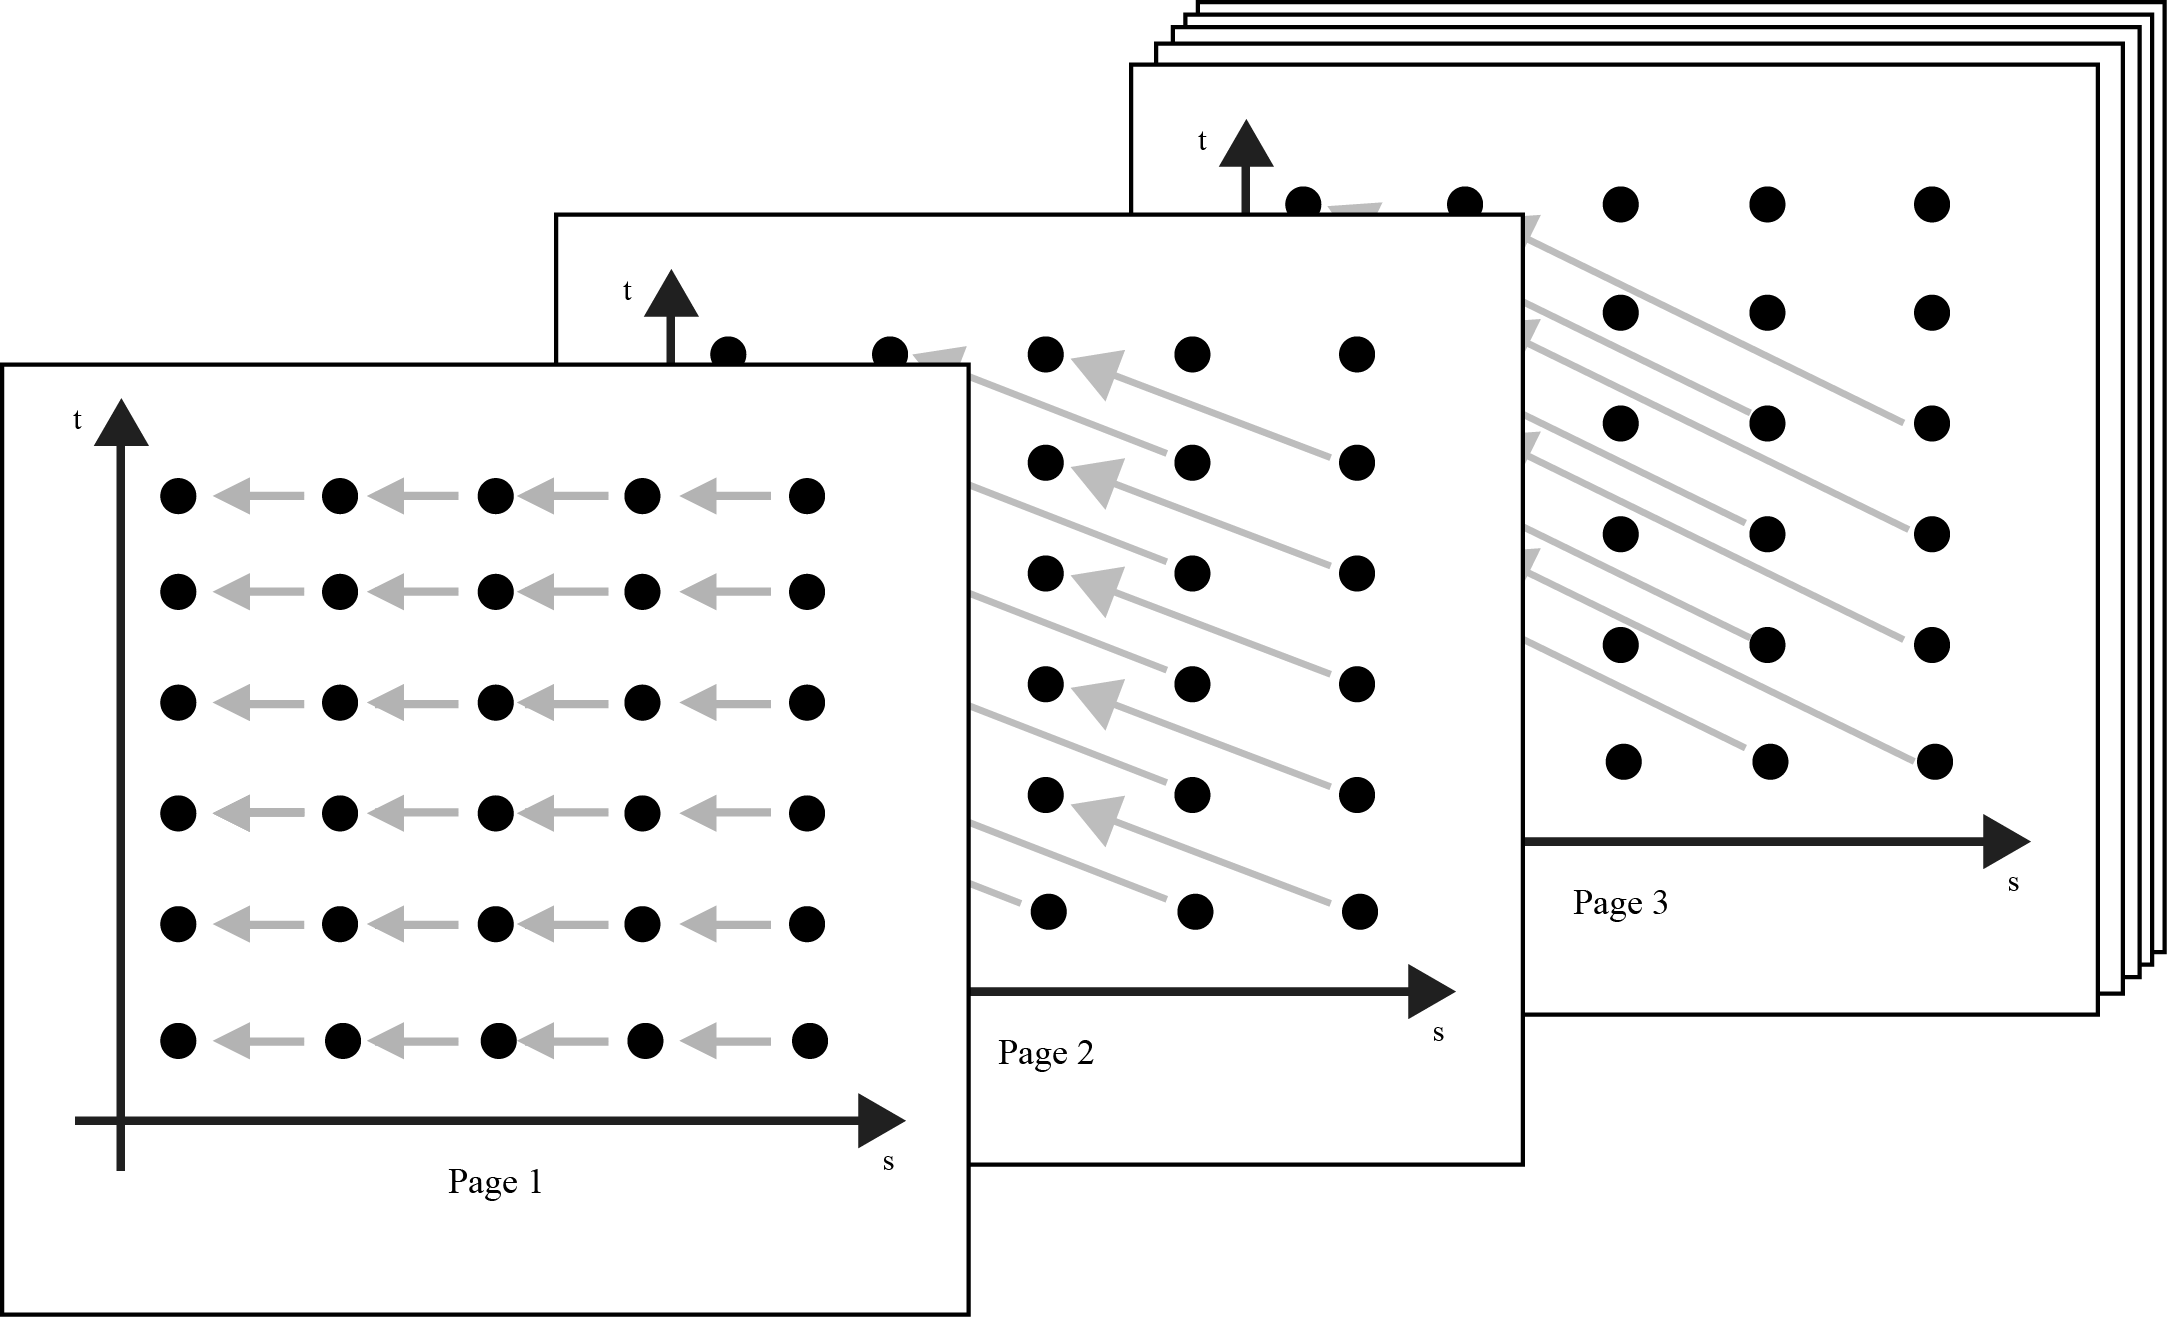
\includegraphics[width=\linewidth,height=0.45\textheight,keepaspectratio]{figures/cover.png}
  \end{center}
       \begin{minipage}{.35\linewidth}
    \begin{flushleft}
      \vspace{2em}
      {\fontsize{6pt}{2pt} \textit{Notes: These are notes live-tex'd
from a graduate course in Algebraic Number Theory taught by Paul Pollack
at the University of Georgia in Spring 2021. As such, any errors or
inaccuracies are almost certainly my own. } } \\
    \end{flushleft}
    \end{minipage}
    \hfill
    \begin{minipage}{.65\linewidth}
    \end{minipage}
  }







\begin{document}

\date{}
\author{D. Zack Garza}
\maketitle
\begin{flushleft}
\textit{D. Zack Garza} \\
\textit{University of Georgia} \\
  \textit{\href{mailto: dzackgarza@gmail.com}{dzackgarza@gmail.com}} \\
{\tiny \textit{Last updated:} 2021-01-17 }
\end{flushleft}


\newpage

% Note: addsec only in KomaScript
\addsec{Table of Contents}
\tableofcontents
\newpage

\def\contradiction
{
\tikz[baseline, x=0.2em, y=0.2em, line width=0.04em]
\draw (0,0) -- ({4*cos(45)},{4*sin(45)})
    (-1,1) -- ({-1 + 4*cos(45)},{1 + 4*sin(45)})
    (-1,3) -- ({-1 + 4*cos(315)},{3 + 4*sin(315)})
    (0,4) -- ({0 + 4*cos(315)},{4 + 4*sin(315)});
}

\hypertarget{thursday-january-14}{%
\section{Thursday, January 14}\label{thursday-january-14}}

See website for notes on books, intro to class.

\begin{itemize}
\item
  Youtube Playlist:
  \url{https://www.youtube.com/playlist?list=PLA0xtXqOUji8fjQysx4k8a6h-hOZ7x5ue}
\item
  Free copies of textbook:
  \url{https://www.dropbox.com/sh/rv5j222kn74bjhm/AABZ1qcR1rOnpaBsa5CL3P_Ea?dl=0\&lst=}
\item
  Course website: ?
\end{itemize}

Paul's description of the course:

``This course is an introduction to arithmetic''beyond
\({\mathbb{Z}}\)``, specifically arithmetic in the ring of''integers" in
a finite extension of \({\mathbb{Q}}\). (Among many other things) we'll
prove three important theorems about these rings:

\begin{itemize}
\tightlist
\item
  Unique factorization into ideals.
\item
  Finiteness of the group of ideal classes.
\item
  Dirichlet's theorem on the structure of the unit group."
\end{itemize}

\hypertarget{motivation}{%
\subsection{Motivation}\label{motivation}}

Solving Diophantine equations, i.e.~polynomial equations over
\({\mathbb{Z}}\).

\begin{example}[?]

Consider \(y^2 = x^3 + x\).

\begin{claim}

\((x, y) = (0, 0)\) is the only solution.

\end{claim}

To see this, write \(y^2 = x(x^2+1)\), which are relatively prime,
i.e.~no \(D\in {\mathbb{Z}}\) divides both of them. Why? If
\(d \divides x\) and \(d \divides x+1\), then
\(d\divides (x^2+1) + (-x) = 1\). It's also the case that both \(x^2+1\)
and \(x^2\) are squares (up to a unit), so \(x^2, x^2 + 1\) are
consecutive squares in \({\mathbb{Z}}\). But the gaps between squares
are increasing: \(1, 2, 4, 9, \cdots\). The only possibilities would be
\(x=0, y=1\), but in this case you can conclude \(y=0\).

\end{example}

\begin{example}[Fermat]

Consider \(y^2 = x^3-2\).

\begin{claim}

\((3, \pm 5)\) are the only solutions.

\end{claim}

Rewrite
\begin{align*}
x^3 = y^2+2 &= (y+ \sqrt{-2})(y - \sqrt{-2}) \\ 
&\in
{\mathbb{Z}}[\sqrt{-2}] \coloneqq\left\{{a+b\sqrt{-2} {~\mathrel{\Big|}~}a,b,\in {\mathbb{Z}}}\right\} \leq {\mathbb{C}}
.\end{align*}
This is a subring of \({\mathbb{C}}\), and thus at least an integral
domain. We want to try the same argument: showing the two factors are
relatively prime. A little theory will help here:

\begin{definition}[Norm Map]

For \(\alpha\in {\mathbb{Z}}[\sqrt{-2}]\) define
\(N \alpha = \alpha\mkern 1.5mu\overline{\mkern-1.5mu\alpha\mkern-1.5mu}\mkern 1.5mu\).

\end{definition}

\begin{lemma}[?]

Let \(\alpha, \beta \in {\mathbb{Z}}[\sqrt{-2}]\). Then

\begin{enumerate}
\def\labelenumi{\arabic{enumi}.}
\item
  \(N(\alpha \beta) = N(\alpha) N(\beta)\)
\item
  \(N( \alpha) \in {\mathbb{Z}}_{\geq 0}\) and \(N(\alpha) = 0\) if and
  only if \(\alpha= 0\).
\item
  \(N(\alpha) = 1 \iff \alpha\in R^{\times}\)
\end{enumerate}

\end{lemma}

\begin{proof}[?]

\begin{enumerate}
\def\labelenumi{\arabic{enumi}.}
\item
  Missing, see video (10:13 AM).
\item
  \(N(\alpha) = a^2 + 2b^2 \geq 0\), so this equals zero if and only if
  \(\alpha= \beta= 0\)
\item
  Write
  \(1 = \alpha\mkern 1.5mu\overline{\mkern-1.5mu\alpha\mkern-1.5mu}\mkern 1.5mu\)
  if \(N(\alpha) = 1 \in R^{\times}\). Conversely if
  \(\alpha\in R^{\times}\) write \(\alpha \beta = 1\), then
  \begin{align*} 
  1 = N(1) = N(\alpha \beta) = N(\alpha ) N(\beta ) \in {\mathbb{Z}}_{\geq 0} 
  ,\end{align*}
  which forces both to be 1.
\end{enumerate}

\end{proof}

\begin{claim}

The two factors \(y \pm \sqrt 2\) are \emph{coprime} in
\({\mathbb{Z}}[\sqrt{-2}]\), i.e.~every common divisor is a unit.

\end{claim}

\begin{proof}[?]

Suppose \(\delta\divides y\pm \sqrt{-2}\), then
\(y + \sqrt{-2} = \delta \beta\) for some
\(\beta\in {\mathbb{Z}}[\sqrt{-2}]\). Take norms to obtain
\(y^2 + 2 = N \delta N \beta\), and in particular

\begin{itemize}
\tightlist
\item
  \(N \delta y^2 +2\)
\item
  \(\delta \divides (y+ \sqrt{-2} ) - (y - \sqrt{-2} ) = 2 \sqrt{-2}\)
  and thus \(N \delta \divides N(2 \sqrt{-2} ) = 8\).
\end{itemize}

In the original equation \(y^2 = x^3-2\), if \(y\) is even then \(x\) is
even, and \(x^3 - 2 \equiv 0-2 \pmod 4 \equiv 2\), and so
\(y^2 \equiv 2 \pmod 4\). But this can't happen, so \(y\) is odd, and
we're done: we have \(N \delta\divides 8\) which is even or 1, but
\(N \delta\divides y^2 +2\) which is odd, so \(N \delta = 1\).

\end{proof}

We can identify the units in this ring:
\begin{align*}
{\mathbb{Z}}[\sqrt{-2} ]^{\times}= \left\{{ a + b \sqrt{-2} {~\mathrel{\Big|}~}a^2 + 2b^2 = 1}\right\}
\end{align*}
which forces \(a^2 \leq 1, b^2 \leq 1\) and thus this set is
\(\left\{{\pm 1}\right\}\).

So we have \(x^3 = ab\) which are relatively primes, so \(a,b\) should
also be cubes. We don't have to worry about units here, since \(\pm 1\)
are both cubes. So e.g.~we can write
\begin{align*}
y + \sqrt{-2} = (a + b \sqrt{-2} )^3 = (a^3-6ab^2) + (3a^2b -2b^3) \sqrt{-2}
.\end{align*}
Comparing coefficients of \(\sqrt{-2}\) yields
\begin{align*} 1 = b(3a^2b - 2b^2) \in {\mathbb{Z}}\implies b \divides 1
,\end{align*}
and thus \(b\in {\mathbb{Z}}^{\times}\),
i.e.~\(b\in \left\{{\pm 1}\right\}\). By cases:

\begin{itemize}
\item
  If \(b=1\), then \(1 = 3a^2 -2 \implies a^2 = 1 \implies a = \pm 1\).
  So
  \begin{align*}
  y = \sqrt{-2} = (\pm 1 + \sqrt{-2} )^3 = \pm 5 + \sqrt{-2}
  ,\end{align*}
  which forces \(y=\pm 5\), the solution we already knew.
\item
  If \(b = -1\), then \(1 = -(3a^2 - 1)\) which forces
  \(1=3a^2 \in {\mathbb{Z}}\), so there are no solutions.
\end{itemize}

\end{example}

\begin{example}[?]

Consider \(y^2 = x^3 - 26\). Rewrite this as
\begin{align*}
x^3 = y^2 + 26 = (y + \sqrt{-26} )(y - \sqrt{-26} )
,\end{align*}
then the same lemma goes through with \(2\) replaced by \(26\)
everywhere where the RHS factors are still coprime. Setting
\(y + \sqrt{-26} = (a + b \sqrt{-26} )^3\) and comparing coefficients,
you'll find \(b=1, a = \pm 3\). This yields \(x=35, y=\pm 207\). But
there are more solutions: \((x, y) = (3, \pm 1)\)! The issue is that we
used unique factorization when showing that \(ab\) is a square implies
\(a\) or \(b\) is a square (say by checking prime factorizations and
seeing even exponents). In this ring, we can have \(ab\) a cube with
\emph{neither} \(a,b\) a cube, even up to a unit.

\end{example}

\begin{question}

When does a ring admit unique factorization? Do you even \emph{need} it?

\end{question}

This will lead to a discussion of things like the \textbf{class number},
which measure the failure of unique factorization. In general, the above
type of proof will work when the class number is 3!

\addsec{ToDos}
\listoftodos[List of Todos]
\cleardoublepage

% Hook into amsthm environments to list them.
\addsec{Definitions}
\renewcommand{\listtheoremname}{}
\listoftheorems[ignoreall,show={definition}, numwidth=3.5em]
\cleardoublepage

\addsec{Theorems}
\renewcommand{\listtheoremname}{}
\listoftheorems[ignoreall,show={theorem,proposition}, numwidth=3.5em]
\cleardoublepage

\addsec{Exercises}
\renewcommand{\listtheoremname}{}
\listoftheorems[ignoreall,show={exercise}, numwidth=3.5em]
\cleardoublepage

\addsec{Figures}
\listoffigures
\cleardoublepage


\printbibliography[title=Bibliography]


\end{document}
